\section{Цель работы и теоретические сведения}

Цель работы --- реализовать метод \(k\) ближайших соседей для классификации
вин и регрессии показателя прогрессирования диабета, сравнить число соседей
и метрики расстояния на валидационной выборке, затем оценить выбранные модели
на тестовой выборке.

При обучении kNN сохраняет признаки и ответы обучающих объектов. Для каждого
нового объекта алгоритм вычисляет расстояния до обучающих точек, упорядочивает
их и выбирает первые \(k\) соседей. При классификации прогнозом служит класс
с наибольшим числом голосов. При регрессии прогноз равен среднему ответу
\(\hat y=k^{-1}\sum_{i\in\mathcal N_k(x)}y_i\), где \(\mathcal N_k(x)\)
обозначает множество выбранных соседей.

Для векторов признаков \(x,z\in\mathbb R^p\) использованы три расстояния:
\[
\begin{aligned}
 d_2(x,z) &= \sqrt{\sum_{j=1}^{p}(x_j-z_j)^2}
 &&\text{(евклидово)},\\
 d_1(x,z) &= \sum_{j=1}^{p}|x_j-z_j|
 &&\text{(манхэттенское)},\\
 d_\infty(x,z) &= \max_{1\le j\le p}|x_j-z_j|
 &&\text{(Чебышёва)}.
\end{aligned}
\]
В \(L_2\) крупные отклонения получают больший вклад из-за возведения в квадрат.
В \(L_1\) абсолютные отклонения суммируются, а \(L_\infty\) учитывает только
максимальное отклонение. Увеличение \(k\) обычно сглаживает прогнозы, снижая
их чувствительность к отдельным наблюдениям.

\section{Разбиение и предварительная обработка}

На первом шаге выделены около \(40\,\%\) объектов с \texttt{random\_state=42}.
Эта часть поровну разбита на валидацию и тест с \texttt{random\_state=43}.
Для Wine оба разбиения стратифицированы по целевому классу, для Diabetes
использовано случайное разбиение. Размеры выборок приведены в таблице ниже.
Доли близки к \(60/20/20\,\%\) с учётом целого числа объектов.

\begin{table}[!ht]
\centering\small
\caption{Размеры выборок и распределение классов Wine}
\begin{tabular}{lrrrr}
\toprule
Набор & Всего & Обучение & Валидация & Тест \\
\midrule
Wine & 178 & 106 & 36 & 36 \\
\quad Класс 0 & 59 & 35 & 12 & 12 \\
\quad Класс 1 & 71 & 42 & 14 & 15 \\
\quad Класс 2 & 48 & 29 & 10 & 9 \\
Diabetes & 442 & 265 & 88 & 89 \\
\bottomrule
\end{tabular}
\end{table}

Оба набора содержат конечные значения во всех столбцах. Каждый признак
стандартизован по формуле \(z_j=(x_j-\mu_j)/\sigma_j\).
Среднее \(\mu_j\) и стандартное отклонение \(\sigma_j\) с делением на
число объектов вычислены по обучающей выборке. Эти же параметры применены
к валидации и тесту. При \(\sigma_j=0\) делитель заменяется единицей.
Целевые значения сохраняют исходный масштаб.

\clearpage
\section{Описательная статистика}

Статистика рассчитана для исходных значений по каждому набору целиком.
Она используется для описания данных. В таблицах \(s\) обозначает
выборочное стандартное отклонение с делением на \(n-1\), а \(Q_1\) и \(Q_3\)
соответствуют 25-му и 75-му процентилям.

\subsection{Wine}

В наборе 178 объектов, 13 химических признаков и три класса вина.
На класс 0 приходится \(33{,}1\,\%\) наблюдений, на класс 1 --- \(39{,}9\,\%\),
на класс 2 --- \(27{,}0\,\%\). Различие масштабов видно по признакам
\texttt{proline} и \texttt{hue}, для которых \(s\) равно \(314{,}907\)
и \(0{,}229\) соответственно.

\experimenttable{Описательная статистика признаков Wine}{wine_statistics}
\experimentfigure{0.98}{wine_distributions.pdf}{Распределения признаков и частоты классов Wine}

\clearpage
\subsection{Diabetes}

В наборе 442 наблюдения и 10 исходных признаков, среди которых возраст,
индекс массы тела, артериальное давление и лабораторные показатели.
Вызов \texttt{load\_diabetes(scaled=False)} возвращает признаки в исходном
масштабе. Переменная \texttt{sex} представлена кодами 1 и 2.
Целевой показатель характеризует прогрессирование болезни через год
и принимает значения от 25 до 346.

\experimenttable{Описательная статистика признаков и целевой переменной Diabetes}{diabetes_statistics}
\experimentfigure{0.98}{diabetes_distributions.pdf}{Распределения признаков и целевого показателя Diabetes}

\clearpage
\section{Реализация алгоритма и метрик}
\subsection{Класс KNN}

Метод \texttt{fit} сохраняет обучающие данные, а \texttt{predict} выбирает
соседей. При равных расстояниях сохраняется порядок обучающих строк.
При равенстве голосов выигрывает класс с наименьшей суммой расстояний
до проголосовавших за него соседей, при равенстве сумм --- наименьшая метка.

\VerbatimInput[fontsize=\codefont,baselinestretch=1,numbers=left,numbersep=7pt,xleftmargin=19pt]{../src/knn.py}

\clearpage
\subsection{Метрики качества}

В матрице ошибок строки соответствуют фактическим классам, столбцы ---
предсказанным. Доля правильных ответов (accuracy) равна сумме диагональных
элементов, делённой на объём выборки. Для каждого класса \(c\) вычислены
\[
 P_c=\frac{TP_c}{TP_c+FP_c},\qquad
 R_c=\frac{TP_c}{TP_c+FN_c},\qquad
 F_{1,c}=\frac{2P_cR_c}{P_c+R_c}.
\]
При нулевом знаменателе соответствующая оценка принимается равной нулю.
Macro-метрики --- арифметические средние \(P_c\), \(R_c\) и \(F_{1,c}\)
по классам. Для регрессии \(e_i=y_i-\hat y_i\), а \(\bar y\) ---
среднее фактическое значение в оцениваемой выборке:
\[
\mathrm{MAE}=\frac{1}{n}\sum_i|e_i|,\qquad
\mathrm{MSE}=\frac{1}{n}\sum_i e_i^2,\qquad
R^2=1-\frac{\sum_i e_i^2}{\sum_i(y_i-\bar y)^2}.
\]

\VerbatimInput[fontsize=\footnotesize,baselinestretch=0.94,numbers=left,numbersep=7pt,xleftmargin=19pt]{../src/metrics.py}

\clearpage
\section{Подбор гиперпараметров}

Для каждой задачи проверены 12 комбинаций \(k\in\{3,5,10,15\}\) и трёх
расстояний. Для Wine выбран максимум macro-F1, для Diabetes --- минимум MSE.
При равенстве целевой метрики приоритет получает меньшее \(k\), затем
порядок \(L_2,L_1,L_\infty\). Жирным шрифтом выделена выбранная строка.

\subsection{Классификация Wine}

\experimenttable{Метрики классификации на валидационной выборке}{wine_validation}
\experimentfigure{0.84}{wine_validation.pdf}{Зависимость macro-F1 от числа соседей для Wine}

При \(L_2\) значение macro-F1 выросло с \(0{,}9743\) при \(k=3,5\) до
\(1{,}0000\) при \(k=10,15\). Манхэттенское расстояние дало тот же максимум
при \(k=5\), поэтому выбрана эта конфигурация. При \(L_1\) дальнейшее
увеличение \(k\) ухудшило оценку до \(0{,}9487\) при \(k=15\).
Расстояние Чебышёва уступило двум другим при всех четырёх значениях \(k\).

\clearpage
\subsection{Регрессия Diabetes}

\experimenttable{Метрики регрессии на валидационной выборке}{diabetes_validation}
\experimentfigure{0.84}{diabetes_validation.pdf}{Зависимость MSE от числа соседей для Diabetes}

Для \(L_\infty\) MSE последовательно снизилась с \(3625{,}56\) при \(k=3\)
до \(2784{,}04\) при \(k=15\). Евклидово расстояние дало свой минимум
\(2849{,}78\) при \(k=3\), а манхэттенское --- \(2995{,}88\) при \(k=10\).
Евклидова модель с \(k=3\) также дала наименьшую MAE (\(42{,}46\)).
По принятому критерию MSE выбрана модель с расстоянием Чебышёва и \(k=15\).

\clearpage
\section{Итоговая оценка на тестовой выборке}

На тесте оценена одна конфигурация для каждой задачи. Обучающая выборка
и параметры стандартизации остались теми же, что при валидации.

\begin{table}[!ht]
\centering\small
\caption{Метрики выбранной модели Wine, \(k=5\), \(L_1\), \(n=36\)}
\begin{tabular}{rrrr}
\toprule
Accuracy & Macro-precision & Macro-recall & Macro-F1 \\
\midrule
\(0{,}9444\) & \(0{,}9410\) & \(0{,}9556\) & \(0{,}9453\) \\
\bottomrule
\end{tabular}
\end{table}

\begin{table}[!ht]
\centering\small
\caption{Метрики выбранной модели Diabetes, \(k=15\), \(L_\infty\), \(n=89\)}
\begin{tabular}{rrr}
\toprule
MAE & MSE & \(R^2\) \\
\midrule
\(45{,}90\) & \(3305{,}46\) & \(0{,}4278\) \\
\bottomrule
\end{tabular}
\end{table}

\begin{figure}[!ht]
    \centering
    \begin{minipage}[t]{0.46\linewidth}
    \centering
    \vspace{0pt}
    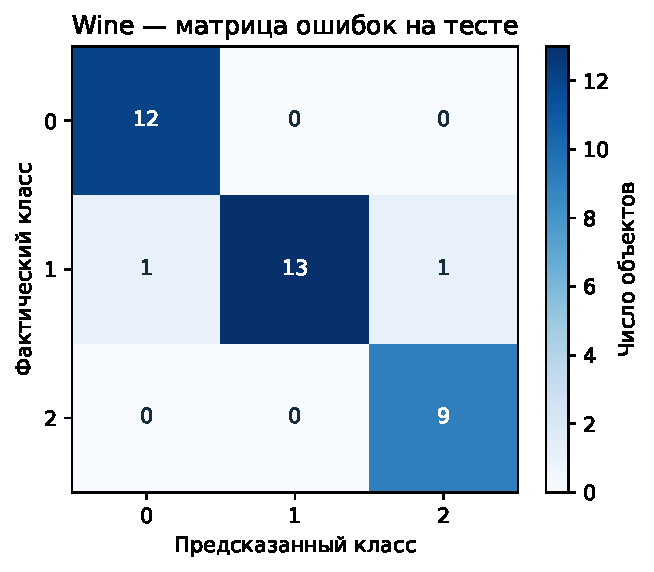
\includegraphics[width=\linewidth]{wine_test.pdf}
    \end{minipage}\hfill
    \begin{minipage}[t]{0.46\linewidth}
    \centering
    \vspace{0pt}
    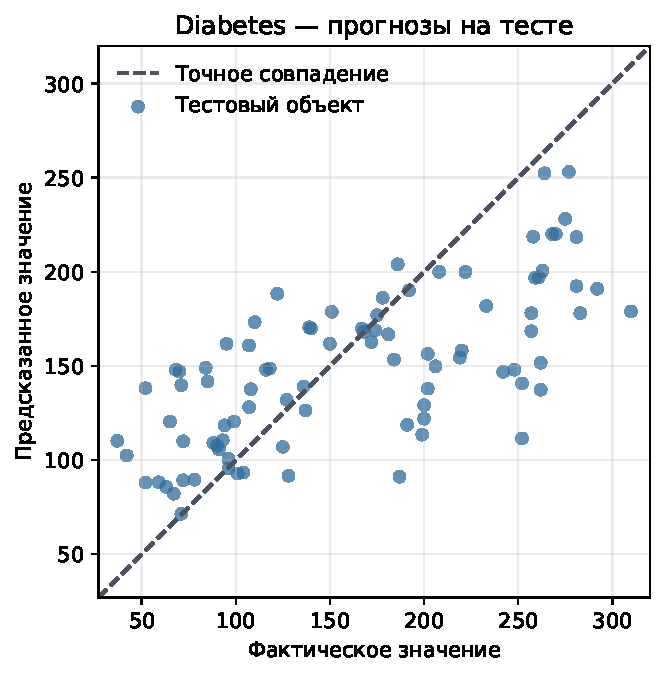
\includegraphics[width=\linewidth]{diabetes_test.pdf}
    \end{minipage}
    \caption{Матрица ошибок Wine и сравнение фактических значений с прогнозами Diabetes}
\end{figure}

Модель Wine верно классифицировала 34 из 36 объектов. Обе ошибки допущены
для объектов класса 1. Один объект отнесён к классу 0, другой --- к классу 2.

Для Diabetes положительное \(R^2\) означает, что сумма квадратов ошибок
модели ниже, чем при прогнозировании средним фактическим значением теста.
Прогнозы лежат в диапазоне от \(71{,}4\) до \(253{,}1\), а фактические
ответы --- от \(37\) до \(310\). При больших фактических значениях часть
точек заметно ниже диагонали. Такая картина согласуется со сглаживанием
прогноза при усреднении по 15 соседям.

\section{Заключение}

На выбранном разбиении Wine модель с \(L_1\) и \(k=5\) получила на тесте
macro-F1 \(0{,}9453\). Для Diabetes модель с \(L_\infty\) и \(k=15\)
дала MSE \(3305{,}46\) и \(R^2=0{,}4278\). В классификации
увеличение \(k\) улучшило macro-F1 для \(L_2\), тогда как для \(L_1\)
максимум достигнут при промежуточном \(k\). В регрессии монотонное
снижение MSE с ростом \(k\) наблюдалось для \(L_\infty\).
Эти результаты отражают совместное влияние числа соседей и расстояния
при фиксированном разбиении данных.
